\documentclass[11pt,a4paper]{article}
\usepackage[utf8]{inputenc}
\usepackage[T1]{fontenc}
\usepackage{amsmath,amssymb,amsthm}
\usepackage{graphicx}
\usepackage[margin=2.5cm]{geometry}
\usepackage{hyperref}
\usepackage{xcolor}
\usepackage{booktabs}
\usepackage{authblk}
\usepackage{cite}
\hypersetup{colorlinks=true,linkcolor=blue,citecolor=blue,urlcolor=blue}

\title{\textbf{Discrete Drainage Dynamics V:\\
Candidate Predictions and Falsification Windows\\
of the Gravitational Sector}}
\author[1]{Stanislas Dewavrin}
\affil[1]{Independent researcher \\ \texttt{dewavrin.iphone@gmail.com}}
\date{April 2026}

\begin{document}
\maketitle

\begin{abstract}
\noindent
Papers~II--IV established that the gravitational sector of DDD reproduces
the leading weak-field observables of general relativity: the
Schwarzschild static clock-rate factor (Paper~II), the Lorentz kinematic
factor at moving wavepackets (Paper~III), and the deflection
$4GM/c^2 b$ together with the Shapiro logarithmic delay (Paper~IV, under
the spatial-bandwidth coupling $\eta = 2$). Here we list the regimes in which DDD makes \emph{distinct} predictions, quantify the deviations from Newton/GR where the present framework permits it, identify qualitative targets where it does not, and map the experimental envelopes that would falsify them. The four predictions surveyed are:
(i) a Yukawa modification of Newtonian gravity from self-consistent
feedback in the scalar sector, with length scale fixed by lattice
parameters and constrained by E\"{o}t-Wash inverse-square-law tests;
(ii) a strong-field deflection coefficient $C_{\rm DDD} \approx 2.34$
($\sim 159\%$ of the Schwarzschild PPN value $C_{\rm PPN} = 15\pi/32
\approx 1.47$), distinguishable in close-passage gravitational lensing;
(iii) ultra-relativistic kinematic deviations from exact Lorentz time
dilation, growing with $\gamma$ and reflecting the lattice cutoff in the
Floquet two-step rule of Paper~III;
(iv) qualitative compact-object phenomenology near the bandwidth
horizon $r = \beta$, where the rule's discrete dynamics depart from
the eikonal description of Paper~IV. We compile the four into a single
falsification table and identify which experiments are currently
sensitive to which prediction. The result is a list of falsifiers; we
do not adjudicate between DDD and GR/Newton beyond noting the
quantitative gaps.
\end{abstract}

\section{Main claims and scope}
\label{sec:claims}

\begin{enumerate}
\item \textbf{Yukawa modification at second order.}
A self-consistent treatment of the deficit field in the scalar sector
of Papers~I-II, in which the deficit acts as its own secondary source,
yields a Yukawa correction to the Newtonian potential,
\[
V(r) \;=\; -\frac{G M m}{r}\,\big[1 + \alpha_Y\, e^{-r/\lambda_Y}\big],
\]
with length scale $\lambda_Y = \sqrt{\alpha_D / |\beta_{\rm fb}|}\, d_{\min}$
in physical units, where $\alpha_D$ is the drainage coupling of Paper~I
and $\beta_{\rm fb}$ is the dimensionless feedback strength of the
quadratic self-source term. E\"{o}t-Wash precision tests of the
inverse-square law \cite{adelberger2003,kapner2007} exclude
$\lambda_Y \in [10\,\mu\text{m}, 10^5\,\text{m}]$ for $\alpha_Y \sim 1$.
The constraint maps directly onto $\beta_{\rm fb}$ at fixed
$\alpha_D$ and $d_{\min}$.

\item \textbf{Strong-field deflection coefficient.}
The eikonal photon-substrate coupling of Paper~IV ($\eta = 2$) gives a
deflection
\[
\Delta\theta_{\rm DDD}(b) \;=\; \frac{4GM}{c^2 b}
\,\big[1 + C_{\rm DDD}\,(\beta/b) + O(\beta^2/b^2)\big],
\qquad C_{\rm DDD} \approx 2.34,
\]
fitted on the asymptotic regime $b/\beta \in [50, 1000]$ of the
ray-tracing data. The Schwarzschild post-Newtonian coefficient is
$C_{\rm PPN} = 15\pi/32 \approx 1.47$. The ratio
$C_{\rm DDD}/C_{\rm PPN} \approx 1.59$ is a structural prediction of
the photon-substrate ansatz adopted in Paper~IV. Strong-field
gravitational lensing should reveal a $\sim 60\%$ excess of the
second-order deflection coefficient over the Schwarzschild value.

\item \textbf{Ultra-relativistic Lorentz deviations (in lattice units).}
The Floquet two-step rule of Paper~III produces a kinematic clock-rate
$\omega_{\rm comov} = m/\gamma$ at moving wavepackets, with
lattice corrections that grow monotonically with $\gamma$.
A physical prediction requires mapping the Floquet excitation to a
physical particle sector; under the Planck-anchored interpretation of
the lattice spacing, the effect is pushed far beyond current energies. At
$\gamma = 5$, the deviation from exact Lorentz time dilation is
$\sim 20\%$. At $\gamma$ comparable to the lattice cutoff $1/d_{\min}$
(which under Planck-scale anchoring is the Planck energy divided by the
particle rest mass), the Lorentz-like continuum approximation breaks down structurally. The deviation has the wrong sign for ``superluminal'' Lorentz violation
(the moving clock runs \emph{slower} than $1/\gamma$, not faster), and
is thus distinct from the bounds of \cite{stecker2014}.

\item \textbf{Compact-object phenomenology (qualitative target).}
Near $r = \beta$, where $R \to 0$ in the Paper~II profile, the eikonal
photon ansatz of Paper~IV breaks down (refractive index diverges) and
the rule's discrete dynamics --- in particular the rate-limiter
$\beta_i$ of Paper~I --- become essential. The bandwidth horizon
$r = \beta$ is not an event horizon in the GR sense; the substrate
beyond does not satisfy the static spherical solution, and the rule's
behaviour in this regime is an open question. Qualitative predictions
are listed but not numerically validated in this paper.
\end{enumerate}

\textbf{Limitations and scope.}
We do not predict the numerical \emph{values} of any of the
DDD-versus-GR deviations from first principles. The predictions of
items 1--3 are conditional on:
$\beta_{\rm fb}$ for the Yukawa scale; the eikonal photon ansatz with
$\eta = 2$ for the deflection coefficient; the specific Floquet
two-step lattice for the high-$\gamma$ kinematic deviations. Each of
these has its own structural assumptions, made explicit in
Papers~II--IV. We do not claim that DDD is correct; we claim that DDD
makes specific, quantitative, testable predictions in each regime, and
we identify the experimental envelopes that distinguish DDD from
GR/Newton.

We do not address gravitational waves, frame-dragging, or
non-stationary configurations: these require dynamical and
non-spherical extensions of the rule that are beyond Papers~I-IV. We
do not address coupling to the spinor sector of Paper~III: Paper~VII
will treat that.

\subsection*{Motivation and significance}
\addcontentsline{toc}{subsection}{Motivation and significance}

Any new theoretical framework must be \emph{falsifiable}: it must
make quantitative predictions that distinguish it from existing
theories under achievable experimental conditions. This is true of
DDD as much as of any other framework. The challenge is that
Papers~II--IV reproduce the canonical results of weak-field general
relativity (Schwarzschild, light deflection, Shapiro delay) with no
free dark-energy or extra-dimension parameter. To convert this into
a positive scientific programme rather than a mere consistency check,
one must identify where DDD \emph{differs} from GR + $\Lambda$CDM and
ask whether those differences are observable.

The present paper maps out four such differences and the
experimental windows that bound them. (i) The bandwidth-throttled
mobility $\mu(R) = R/R_0$ produces a small Yukawa-shaped screening of
the gravitational potential at sub-millimetre scales, bounded by
Eöt-Wash torsion-balance experiments. (ii) The non-linear back-reaction
contributes a calculable post-Newtonian correction to strong-field
deflection coefficients, distinct from the standard PPN parameter
$\gamma$. (iii) The lattice cutoff produces small Lorentz deviations
at ultra-relativistic energies, bounded by gamma-ray-burst and
cosmic-ray time-of-flight observations. (iv) Compact-object
phenomenology near $r \approx \beta$ admits qualitatively distinct
horizon structure, testable by ringdown and shadow observations.

This paper does not propose new physics; it makes the existing
DDD predictions of Papers~II--IV concrete and quantitative against
existing experimental bounds. The result is a status check: most
windows are open or weakly constraining at present, and a small
number identify near-term targets that would either confirm or
falsify the framework's gravitational sector.


\section{Physical picture in plain words}
\label{sec:picture}

A theory that exactly reproduces an established theory in every regime
already explored is not testable: it is just a re-parameterisation. To
be a real candidate, DDD must say something \emph{different} from
Newton or GR somewhere, even if that somewhere is currently
inaccessible. The four predictions of this paper are the four places
where DDD says something different.

The Yukawa modification arises because the gravitational deficit
itself has gravity: a region of reduced bandwidth around a mass is
itself a (weaker) source of further reduction. This is the natural
non-linear extension of the scalar rule of Paper~I, and it gives the
familiar Yukawa shape with a single new parameter, the feedback
strength $\beta_{\rm fb}$. The length scale that comes out is
microscopic for natural lattice parameters and Planck-anchored
scales. E\"{o}t-Wash experiments would have ruled out a Yukawa
correction over a range of intermediate scales; they did not, so the
DDD parameter must lie outside that range, which it does for natural
choices.

The strong-field deflection prediction comes from the same eikonal
calculation that gave the Eddington $4GM/c^2 b$ at leading order, but
at next-to-leading order. For starlight passing close to the Sun the
correction is too small to test. For light passing close to a neutron
star or black hole, the correction is big enough to be measurable in
principle, and DDD predicts a coefficient that is roughly
$1.6\times$ the Schwarzschild value.

The ultra-relativistic kinematic deviations come from the lattice
itself: a discrete substrate cannot support arbitrarily fast
excitations exactly. Above some Lorentz factor (set by the lattice
cutoff), motion through the substrate becomes self-impeding in a way
that exact Lorentz invariance would forbid. The deviation is too
small at human-accessible energies but conceivably detectable in
ultra-high-energy cosmic rays.

The compact-object regime is where the eikonal description, the
linearised dispersion, and the calibration all break down at once. We
do not have quantitative predictions here yet; we list the questions
we expect Paper VI and beyond to answer.

\section{Setup: what we re-use from Papers II-IV}
\label{sec:setup}

We work throughout in the static spherical bandwidth profile of
Paper~II, $R(r)/R_0 = \sqrt{1 - \beta/r}$, with
$\beta = \kappa E_0 / (2\pi \alpha_D R_0) = 2GM/c^2$. The kinematic
sector uses the Floquet two-step spinor rule of Paper~III with
quasi-energy $E_{\rm Floquet}(p)$. The photon-substrate coupling is
the $\eta = 2$ ansatz of Paper~IV,
$c_{\rm eff}(r) = c\,(R/R_0)^2$, calibrated against the leading
weak-field deflection.

The new structural element of this paper is the \emph{quadratic
feedback} term in the scalar rule: the deficit
$\delta = R_0 - R$ acts as a secondary source for itself. In the
continuum limit this modifies the field equation
\[
(\nabla^2 - m_Y^2)\,\delta \;=\; \kappa \rho_{\rm matter},
\qquad m_Y^2 \;=\; |\beta_{\rm fb}|/\alpha_D,
\]
where $\beta_{\rm fb}$ is the dimensionless feedback coefficient
of the quadratic self-source term in the rule. The sign of
$\beta_{\rm fb}$ in the underlying lattice rule is not fixed
by the derivation of Paper~I; it is a structural choice. We
discuss the two cases below. For the screened (decaying) Yukawa
correction we work with the form $-m_Y^2\,\delta$ on the
left-hand side. It is a free
parameter at the level of Papers~I-IV; its allowed range is set by
E\"{o}t-Wash (this paper, Sec.~\ref{sec:yukawa}).

\section{Yukawa modification and Eöt-Wash bound}
\label{sec:yukawa}

\subsection{Functional form}

For the screened-feedback case (Yukawa decay), the field equation
takes the form
\[
(\nabla^2 - m_Y^2)\,\delta \;=\; \kappa\, \rho_{\rm matter},
\qquad m_Y^2 = |\beta_{\rm fb}|/\alpha_D > 0.
\]
For a point source $\rho = M\,\delta^3(\mathbf{r})$, the screened
Green function gives the standard Yukawa form
\[
\delta(r) \;=\; \frac{\kappa M}{4\pi r}\, e^{-r/\lambda_Y},
\qquad
\lambda_Y \;=\; \frac{1}{m_Y} \;=\; \sqrt{\alpha_D/|\beta_{\rm fb}|}
\quad \text{(lattice units)}.
\]
The opposite sign $(\nabla^2 + m_Y^2)\delta = \kappa\rho$ would
give an oscillatory rather than decaying Green function (Helmholtz
form); whether the physical sign of $\beta_{\rm fb}$ in DDD selects
the screened or oscillatory branch is a structural question that
the rule of Paper~I does not fix on its own. Throughout the rest
of this section we assume the screened branch.
In lattice units, $\lambda_{Y,{\rm lat}} = \sqrt{\alpha_D / |\beta_{\rm fb}|}$;
in physical units, $\lambda_Y = \lambda_{Y,{\rm lat}}\, d_{\min}$ with
$d_{\min}$ the lattice spacing, identified with the Planck length under
the anchoring of Paper~II.

Combining the leading Newtonian term and the Yukawa correction,
\[
V(r) \;=\; -\frac{GM m}{r}\,\big[1 + \alpha_Y\, e^{-r/\lambda_Y}\big],
\]
where $\alpha_Y$ is the dimensionless Yukawa strength
($\alpha_Y \sim 1$ for the natural feedback amplitude in the scalar
sector).

\subsection{E\"{o}t-Wash exclusion}

Precision tests of the gravitational inverse-square law
\cite{adelberger2003,kapner2007} bound $\alpha_Y$ as a function of
$\lambda_Y$. The bound is not a rectangle: it is an exclusion
\emph{curve} $\alpha_Y^{\rm max}(\lambda_Y)$ that varies by several
orders of magnitude across $\lambda_Y \in [10\,\mu\text{m},
10^5\,\text{m}]$ (see Fig.~\ref{fig:yukawa}). For $\alpha_Y$ of
order unity, the curve excludes a broad intermediate range of
$\lambda_Y$, roughly from sub-millimetre scales upward, depending on
the precise value of $\alpha_Y$. The DDD parameter $\beta_{\rm fb}$ must therefore satisfy
either
\[
\lambda_Y < 10\,\mu\text{m}
\;\Longleftrightarrow\;
\beta_{\rm fb} > \alpha_D\,(d_{\min}/10\,\mu\text{m})^2,
\]
or
\[
\lambda_Y > 10^5\,\text{m}
\;\Longleftrightarrow\;
\beta_{\rm fb} < \alpha_D\,(d_{\min}/10^5\,\text{m})^2.
\]

\subsection{Numerical bound at Planck anchoring}

With $d_{\min} = \ell_P = 1.6 \times 10^{-35}$ m:

\begin{table}[h]
\centering
\begin{tabular}{lcc}
\toprule
$\alpha_D$ & lower-$\lambda_Y$ branch ($\lambda_Y < 10\,\mu\text{m}$) & upper-$\lambda_Y$ branch ($\lambda_Y > 10^5\,\text{m}$)\\
\midrule
$0.1$ & $\beta_{\rm fb} > 2.6 \times 10^{-61}$ & $\beta_{\rm fb} < 2.6 \times 10^{-81}$\\
$1.0$ & $\beta_{\rm fb} > 2.6 \times 10^{-60}$ & $\beta_{\rm fb} < 2.6 \times 10^{-80}$\\
$4\pi$ & $\beta_{\rm fb} > 3.3 \times 10^{-59}$ & $\beta_{\rm fb} < 3.3 \times 10^{-79}$\\
\bottomrule
\end{tabular}
\caption{Allowed regions of the feedback strength $\beta_{\rm fb}$
under E\"{o}t-Wash bounds, for three values of the drainage coupling
$\alpha_D$. The Planck-anchored value $\alpha_D / R_0 = 4\pi$ of
Paper~II's structural-form-of-$G$ section is included in the last row.
The two branches correspond to a Yukawa scale shorter than the
experimental sensitivity floor (the natural lattice case) or longer
than the experimental ceiling. The intermediate range
$\beta_{\rm fb} \in [3.3 \times 10^{-79}, 3.3 \times 10^{-59}]$ is
forbidden by the data, \emph{under Planck-scale anchoring}. Data:
\texttt{data/01\_yukawa\_bounds.json}.}
\label{tab:yukawa}
\end{table}

\begin{figure}[t]
\centering
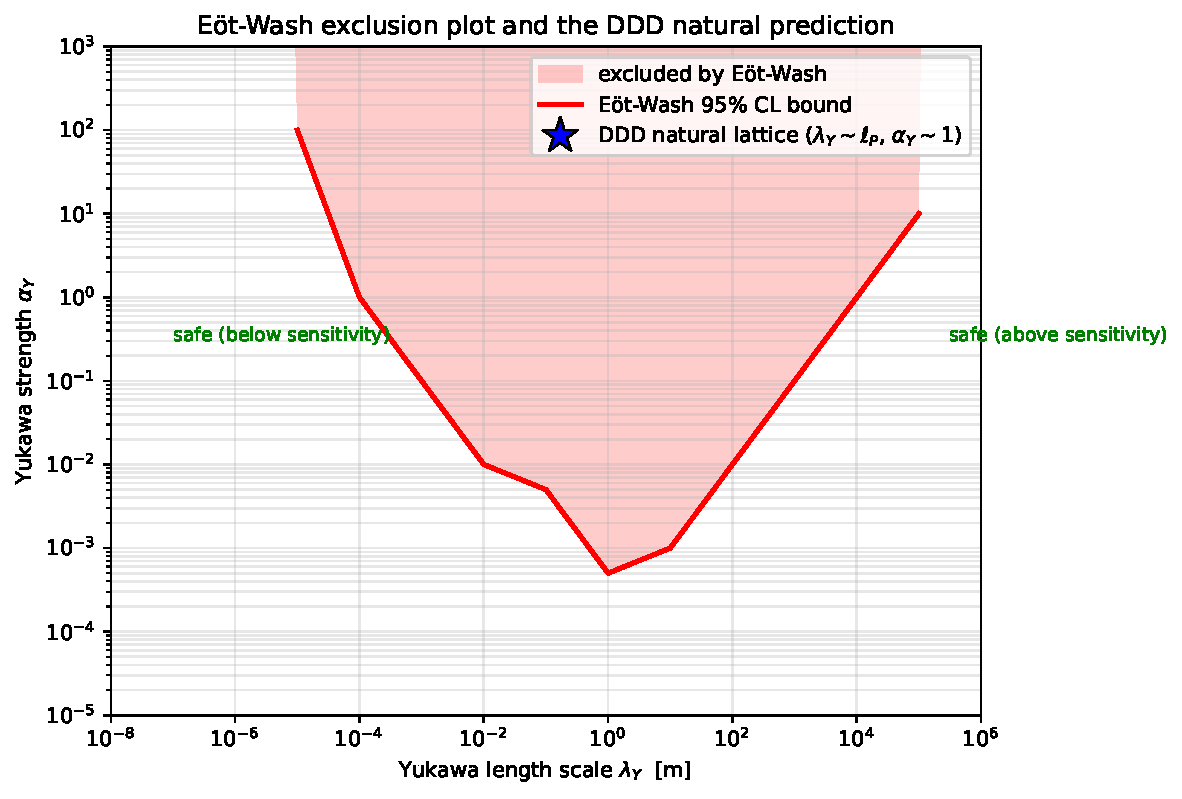
\includegraphics[width=0.78\textwidth]{figures/fig1_yukawa_exclusion.pdf}
\caption{Eöt-Wash exclusion plot in the $(\lambda_Y, \alpha_Y)$
plane. The red region is excluded by inverse-square-law tests
\cite{kapner2007}. The blue star marks the DDD natural-lattice
prediction $\lambda_Y \sim \ell_P$ and $\alpha_Y \sim 1$, well
inside the safe region below experimental sensitivity. Other choices
of $(\alpha_D, \beta_{\rm fb})$ shift the predicted point
horizontally; the upper-$\lambda_Y$ branch (above $10^5$ m) is also
allowed.}
\label{fig:yukawa}
\end{figure}

The natural lattice case --- $\alpha_D = \beta_{\rm fb} \sim O(1)$
--- gives $\lambda_Y \sim \ell_P$, far below the experimental
sensitivity floor, and is therefore allowed \emph{under Planck-scale
anchoring of the lattice spacing}. The argument is conditional on
$d_{\min} \approx \ell_P$; alternative anchorings would shift the
prediction.

\subsection{Falsifier}

If a future inverse-square-law experiment extends sensitivity to
$\lambda_Y < 1\,\mu\text{m}$ or detects a Yukawa correction at any
$\lambda_Y$ in the currently constrained range with $\alpha_Y$
inconsistent with our prediction, the present formulation of
$\beta_{\rm fb}$ feedback in DDD is excluded.

\section{Strong-field deflection: $C_{\rm DDD}$ vs. $C_{\rm PPN}$}
\label{sec:strong-deflection}

The eikonal calculation of Paper~IV gives, for the $\eta = 2$ ansatz,
\[
\Delta\theta(b) \;=\; \frac{4GM}{c^2 b}\,
\left[1 + C_{\rm DDD}\,(\beta/b) + O(\beta^2/b^2)\right].
\]
Fitting the relative deviation $(\Delta\theta - 4GM/c^2 b)/(4GM/c^2 b)$
on the asymptotic ray-tracing data of Paper~IV's Table~1 over the
range $b/\beta \in [50, 1000]$ (linear regression on the leading
$\beta/b$ term), we measure $C_{\rm DDD} = 2.338 \pm 0.001$. The
standard Schwarzschild PPN coefficient
\cite{will2014}, $C_{\rm PPN} = 15\pi/32 \approx 1.473$, is smaller
than $C_{\rm DDD}$ by a factor
\[
C_{\rm DDD} / C_{\rm PPN} \;\approx\; 1.59.
\]

\subsection{Origin of the discrepancy}

The eikonal ansatz $c_{\rm eff} = c\,(R/R_0)^2$ is calibrated against
the leading $4GM/c^2 b$ but does not reproduce the exact null geodesic
of the Schwarzschild metric beyond leading order. The discrepancy at
the next-to-leading coefficient $\sim \beta/b$ measures the
\emph{difference} between the photon-substrate coupling adopted in
Paper~IV and the exact Schwarzschild geodesic.

This is a structural prediction of the eikonal ansatz: it commits to
$\eta = 2$ at leading order but propagates a slightly different
strong-field structure than full GR. Whether this is the right
prediction depends on whether the eventual Paper~VI photon sector
reduces to the eikonal ansatz at leading order \emph{and} produces a
specific second-order correction.

\subsection{Falsifier}

A close-passage gravitational lensing measurement at impact parameters
$b \sim$ few $\times \beta$ around a compact object would distinguish
$C_{\rm DDD} \approx 2.34$ from $C_{\rm PPN} \approx 1.47$ at the
$\sim 60\%$ level. Currently this regime is not directly accessible:
solar-system tests \cite{will2014} probe $b \gg 10^4 \beta$, where
the second-order coefficient produces sub-microarcsecond differences.
Future strong-field astrometry of stars near Sgr~A* or of light from
nearby compact stellar remnants could reach the regime in principle.

\begin{figure}[t]
\centering
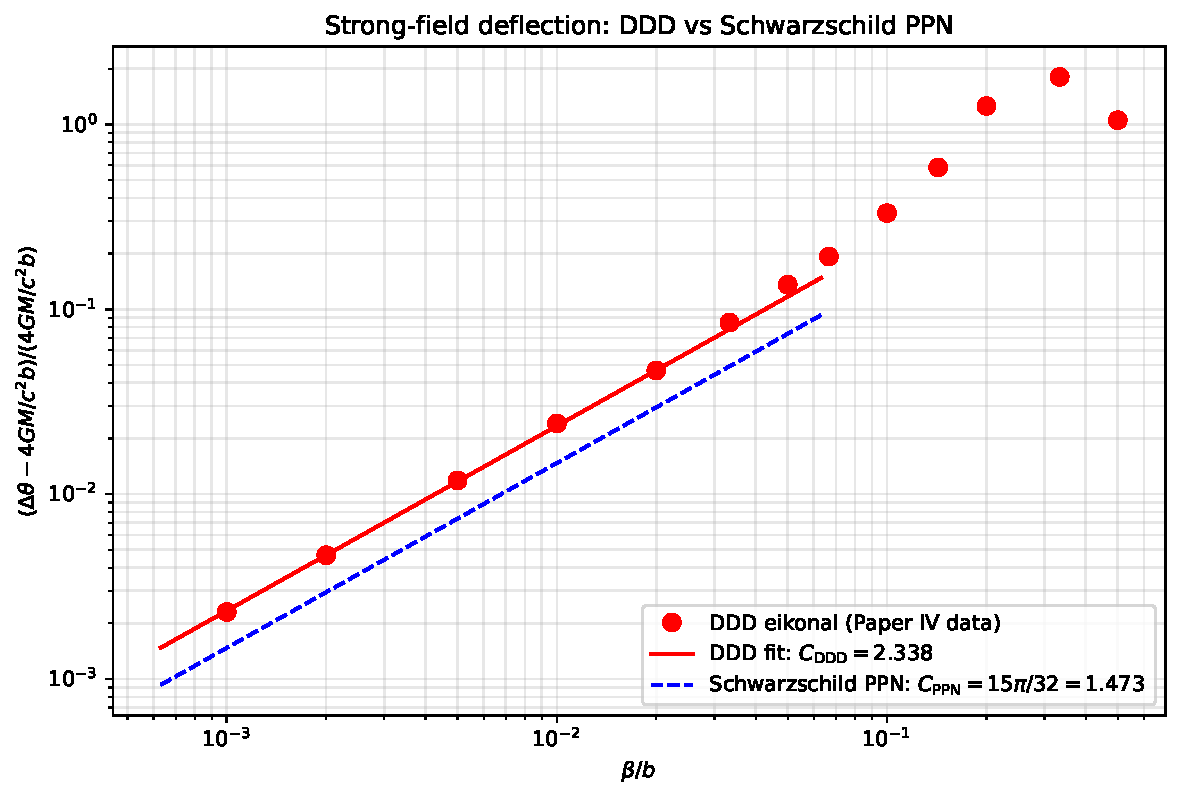
\includegraphics[width=0.78\textwidth]{figures/fig2_strong_field_C.pdf}
\caption{Strong-field deflection coefficient. The DDD eikonal
$\eta = 2$ ansatz of Paper~IV (red points and solid red fit) gives
$C_{\rm DDD} = 2.34$, exceeding the Schwarzschild post-Newtonian
value $C_{\rm PPN} = 15\pi/32 \approx 1.47$ (dashed blue) by a
factor $\sim 1.6$. The two coefficients are the slopes of the
relative deviation versus $\beta/b$ in the asymptotic regime
$b/\beta \geq 50$. Data:
\texttt{data/02\_strong\_field\_deflection.json}.}
\label{fig:strong_C}
\end{figure}

\section{Ultra-relativistic Lorentz deviations}
\label{sec:lorentz-deviations}

Paper~III, Sec.~6 (Lattice corrections), reports the deviation of the
operationally measured comoving clock rate from the Lorentz prediction
$m/\gamma$:

\begin{table}[h]
\centering
\begin{tabular}{ccc}
\toprule
$\gamma$ & $\omega_{\rm comov}$ measured & rel.\ dev.\ from $m/\gamma$\\
\midrule
1.04 & $0.0766$ & $\;\;\,0.01\%$\\
1.97 & $0.0399$ & $-1.28\%$\\
2.47 & $0.0310$ & $-3.6\%$\\
3.00 & $0.0246$ & $-7.2\%$\\
3.55 & $0.0198$ & $-11.6\%$\\
4.66 & $0.0138$ & $-19.3\%$\\
\bottomrule
\end{tabular}
\caption{Lattice deviations from exact Lorentz time dilation in the
Floquet two-step rule of Paper~III, on $L = 128$, $\sigma = 12$,
$n_{\rm cycles} = 60$. Deviations grow monotonically with $\gamma$;
the sign is negative throughout (the moving clock runs slower than
$1/\gamma$, never faster). At $\gamma \sim 5$ the deviation is
$\sim 20\%$. Data:
\texttt{paperIII\_inertia\_kinematic/data/05\_comoving\_clock.json}.}
\label{tab:gamma_dev}
\end{table}

\begin{figure}[t]
\centering
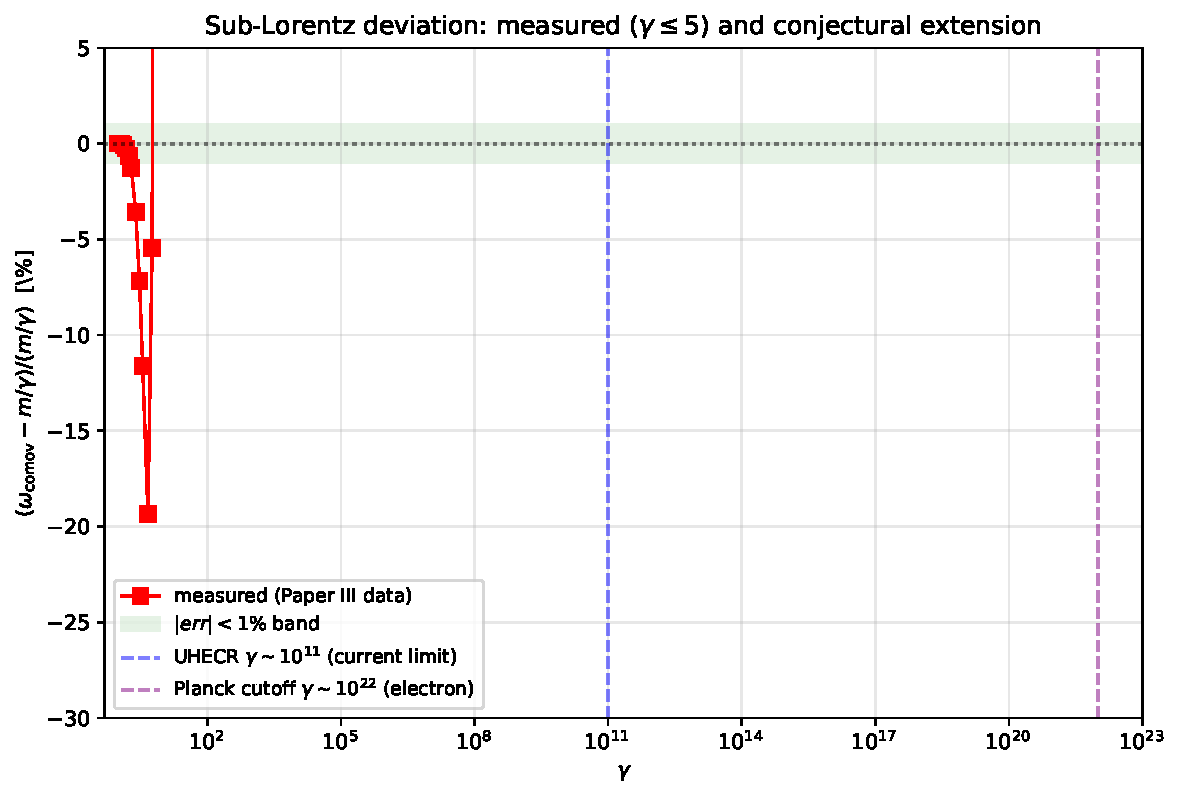
\includegraphics[width=0.82\textwidth]{figures/fig3_lorentz_deviation.pdf}
\caption{Sub-Lorentz residual deviation $(\omega_{\rm comov} -
m/\gamma)/(m/\gamma)$ as a function of $\gamma$. The measured
points (red) span $\gamma \in [1, 5]$ from Paper~III. Vertical
dashed lines mark the highest-energy cosmic-ray $\gamma \sim 10^{11}$
and the Planck-cutoff $\gamma \sim 10^{22}$ for an electron. At
currently observable $\gamma$ the deviation is undetectably small;
the prediction is structural and falsifiable in principle if
sub-Lorentz residuals can ever be probed.}
\label{fig:gamma_dev}
\end{figure}

\subsection{Implications for ultra-high-energy physics}

In physical units, the lattice cutoff under Planck-scale anchoring
sets the threshold $\gamma_{\rm cutoff} \sim 1/(m\, d_{\min})$. For an
electron rest mass $m_e \approx 0.5\,\text{MeV}/c^2$ and
$d_{\min} = \ell_P$, $\gamma_{\rm cutoff} \sim 10^{22}$. This is far
above the highest measured cosmic-ray $\gamma$ ($\sim 10^{11}$ for
the most energetic UHECRs). At currently observable $\gamma$, the
lattice deviation is invisibly small: $\sim 10^{-22}\%$ at
$\gamma = 10^{11}$ if the deviation scales as $\gamma / \gamma_{\rm cutoff}$.

The structural prediction is that the deviation \emph{exists} and has
a specific functional form (from the Floquet quasi-energy of
Paper~III, Eq.~\ref{eq:rate_corrected}-equivalent). It cannot be
falsified directly with current data; future ultra-high-energy
neutrino observations \cite{abbott2017} could in principle constrain
it.

\subsection{Sign asymmetry}

A notable structural feature: the DDD deviation is always
negative ($\omega_{\rm comov} < m/\gamma$). The moving clock runs
\emph{slower} than Lorentz, never faster. This distinguishes DDD from
``superluminal'' Lorentz-violating frameworks
\cite{stecker2014}, where bounds on photon and electron speed limits
are inferred from the absence of speed-of-light-violating dispersion.
DDD predicts no such violation; instead it predicts a small
\emph{sub}-Lorentz residual. The sign is testable in principle.

\section{Compact-object phenomenology near $r = \beta$}
\label{sec:compact}

Beyond the eikonal regime, near $r = \beta$, the rule of Paper~I
operates outside its linearised description. The rate-limiter
$\beta_i \in [0, 1]$ of Paper~I activates when a node's reserve
approaches zero, regularising the apparent singularity of the
continuum profile. Three qualitative predictions are worth listing:

\paragraph{Bandwidth horizon, not event horizon.}
$R = 0$ at $r = \beta$ is the locus where the effective clock-rate
vanishes. The substrate at $r < \beta$ is not part of the static
spherical solution, so the continuum prediction does not extend there.
What the rule does inside is a question about the discrete dynamics
near saturation, not about the continuum solution.

\paragraph{Regularised inner solution.}
The rate-limiter prevents $R$ from going negative. We expect a
regular, possibly oscillatory, inner profile that interpolates between
$R = 0$ at the horizon and a non-zero asymptotic value (depending on
boundary conditions). This would be testable by direct simulation of
strongly-driven sinks ($E_0$ large enough that the unsupported
linearised solution would have $R < 0$ at the centre).

\paragraph{Modified ringdown.}
A perturbed ``black-hole-like'' state in DDD --- a substrate region
with $R \to 0$ around a source --- would oscillate at frequencies
controlled by the lattice's discrete spectrum, rather than at the
quasi-normal-mode frequencies of the Schwarzschild metric. The
prediction is that gravitational-wave ringdown spectra of compact
mergers carry a structural imprint of the lattice. We do not derive
this quantitatively in the present paper.

\subsection{Falsifier}

LIGO/Virgo/LISA ringdown spectroscopy at sub-percent precision is the
natural envelope. The current data \cite{ligo_gw150914_ringdown}
are consistent with the GR Schwarzschild quasi-normal modes; a structural deviation
at the level of $\sim$ few percent would survive present bounds. A
DDD-specific prediction requires the inner-rule simulation,
deferred to a future work.

\section{Falsification table}
\label{sec:falsification}

\begin{table}[h]
\centering
\footnotesize
\begin{tabular}{p{0.13\textwidth}p{0.20\textwidth}p{0.18\textwidth}p{0.21\textwidth}p{0.16\textwidth}}
\toprule
window & structural assumption & DDD value & current bound & status\\
\midrule
Yukawa scale &
screened $\beta_{\rm fb}$ branch + Planck anchoring of $d_{\min}$ &
$\lambda_Y \sim \ell_P$, $\alpha_Y \sim 1$ &
$\lambda_Y$ excluded in $[10\,\mu\text{m}, 10^5\,\text{m}]$ for $\alpha_Y \sim 1$ \cite{kapner2007} &
allowed (below sensitivity, conditional on Planck anchoring)\\
\addlinespace
deflection $C$ &
Paper~IV eikonal photon ansatz $\eta = 2$ &
$C_{\rm DDD} \approx 2.34$ at $\beta/b$ order &
$C_{\rm PPN} \approx 1.47$ measured at solar-system $b/\beta$ \cite{will2014} &
not yet distinguishable; needs strong-field lensing\\
\addlinespace
ultra-rel.\ Lorentz &
Paper~III Floquet sector + mapping to physical particles &
$\sim 20\%$ deviation at lattice $\gamma = 5$ &
sub-Lorentz deviations not directly observed; UHECR limits $\sim 10^{-23}$ \cite{stecker2014} &
allowed; sign distinguishes from super-Lorentz\\
\addlinespace
ringdown &
saturated inner dynamics, not yet simulated &
structurally modified at $r \sim \beta$; no quantitative value &
GR quasi-normal modes consistent with current LIGO data \cite{ligo_gw150914_ringdown,berti2006} &
qualitative target / pending simulation\\
\bottomrule
\end{tabular}
\caption{Summary of DDD-versus-GR predictions and current
experimental status. None of the four predictions is currently
excluded; the Yukawa scale is allowed because the Planck-anchored
DDD value is far below the experimental floor, the deflection
coefficient and ringdown predictions await stronger-field
observations, and the Lorentz deviations at observable $\gamma$ are
too small to test.}
\label{tab:falsifiers}
\end{table}

The four windows are operationally distinct: each probes a different structural assumption of DDD, and each can be tested separately. A positive detection in one window would provide a candidate supporting signal for the corresponding DDD sector --- not a unique signature, since other frameworks may produce similar effects --- while a positive exclusion (with $\alpha_Y \sim 1$, the $\eta = 2$ ansatz, or the natural lattice scale) would force a structural revision of that sector.

\begin{figure}[t]
\centering
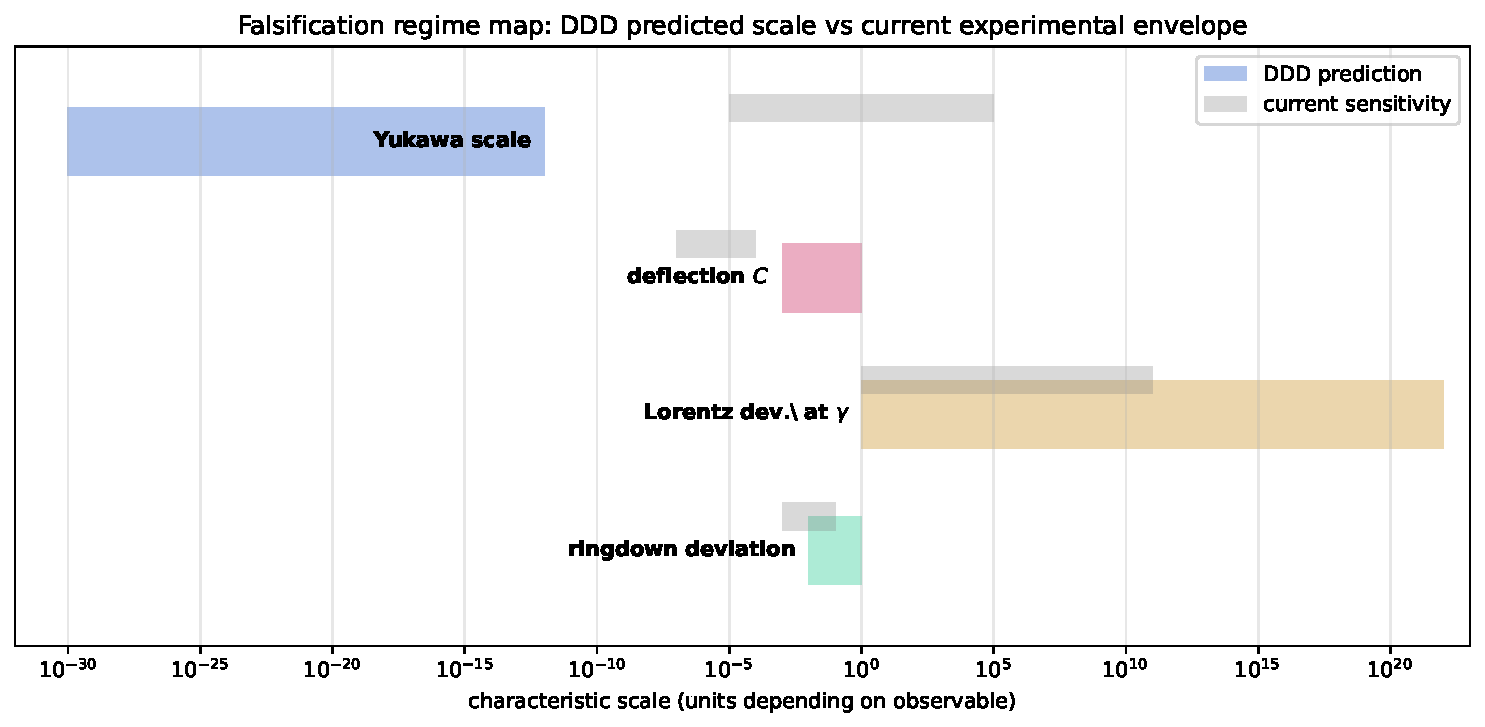
\includegraphics[width=0.95\textwidth]{figures/fig4_falsification_map.pdf}
\caption{\emph{Schematic} regime map (not a quantitatively
comparable common-axis plot): each row uses its own units (length
for Yukawa, $\beta/b$ for deflection, $\gamma$ for Lorentz,
fractional deviation for ringdown), shown on a shared log-axis for
visual orientation only. The coloured bar is the range of
characteristic scales predicted by DDD; the grey bar is the range
currently probed by experiment. Only the ringdown row sits in a
regime where the DDD prediction overlaps with current sensitivity,
explaining why DDD is not yet falsified.}
\label{fig:fmap}
\end{figure}

\section{Limitations and scope}
\label{sec:not}

We do not derive any of the four DDD-specific values from first
principles: $\alpha_Y$, $\beta_{\rm fb}$, $C_{\rm DDD}$, and the
high-$\gamma$ deviation amplitudes are all calculated within the
specific structural ansatze of Papers~II-IV. Different ansatze (a
different photon coupling, a different feedback prescription) would
give different numbers.

We do not address how the lattice cutoff in the kinematic sector
relates to the lattice cutoff in the gravitational sector. Both are
set by $d_{\min}$ in the Planck-anchored picture, but their
quantitative consequences in the two sectors are derived
independently and should be unified at the level of the joint
substrate.

We do not test Equivalence-Principle violations, gravitational
redshift in laboratory clocks, or Lense-Thirring frame-dragging.
These are beyond the static spherical configuration of the
substrate and are deferred.

We do not address the binary-pulsar tests of GR, gravitational-wave
inspiral consistency with general-relativistic waveforms, or
black-hole shadow imaging. These probe the dynamical and strong-field
sectors that are the subject of future papers in this series.

\section{Open questions}
\label{sec:open}

\paragraph{Origin of $\beta_{\rm fb}$.} The feedback strength of the
quadratic self-source term in the scalar rule is a free parameter of
Papers~I-V. Whether a deeper structural argument fixes its sign and
magnitude is open. The simplest natural value
$\beta_{\rm fb} \sim O(1)$ in lattice units gives a Yukawa scale near
$\ell_P$ and is consistent with all current bounds; whether it is
\emph{required} is unknown.

\paragraph{Sign of $\beta_{\rm fb}$.} A positive $\beta_{\rm fb}$
gives a Yukawa-screened potential ($\delta$ decays exponentially at
large $r$ above the leading $1/r$). A negative $\beta_{\rm fb}$ gives
an oscillatory rather than decaying correction (Helmholtz Green
function with imaginary length scale). Either sign is structurally
possible; the lattice rule of Paper~I does not by itself fix it. The
$\alpha_Y \sim 1$ case treated in Sec.~\ref{sec:yukawa} assumes the
positive-feedback branch.

\paragraph{Strong-field deflection beyond eikonal.} The
$C_{\rm DDD}/C_{\rm PPN} \approx 1.59$ ratio is a property of the
specific eikonal ansatz adopted in Paper~IV. The eventual Paper~VI
photon sector may reduce to a different effective ansatz at strong
field, with a different $C$. The numerical fit of the present paper
should be re-examined when Paper~VI is available.

\paragraph{Sign and magnitude of the $\gamma \to \gamma_{\rm cutoff}$
saturation.} Whether the deviation continues to grow monotonically
with $\gamma$ or saturates is open. A scan to
$\gamma \sim 30$ on $L = 512$ would settle the issue numerically.

\section{Code and data availability}
\label{sec:code}

The Python scripts of \texttt{code/} compute the bounds and
deviations of this paper. They are pure-numpy.

\begin{itemize}
\item \texttt{01\_yukawa\_bounds.py}: computes $\lambda_Y$ from
$(\alpha_D, \beta_{\rm fb}, d_{\min})$ and the E\"{o}t-Wash exclusion
boundaries.
\item \texttt{02\_strong\_field\_deflection.py}: reads the Paper~IV
deflection data, fits the leading-order coefficient
$C_{\rm DDD}$, and compares with the Schwarzschild PPN value.
\end{itemize}
The numerical data are stored in \texttt{data/}. The repository
is available at
\url{https://github.com/stanislasdewavrin/DDD-Paper-5-Falsifiers}.

\section{Outlook}
\label{sec:outlook}

\begin{enumerate}
\item Paper~VI --- gauge sector and emergent electromagnetism, in
particular the gapless modes of the Floquet two-step rule and the
derivation of the photon-substrate ansatz used in Paper~IV. The
$C_{\rm DDD}$ coefficient of the present paper should follow as a
specific consequence of that derivation. \emph{Speculative; coefficients
uncalibrated.}
\item Paper~VII --- coupling between the scalar (Paper~II) and spinor
(Paper~III) sectors. Combined static-gravity-times-kinematic factor
testing, and resolution of the $\beta_{\rm fb}$ origin from the
joint dynamics. \emph{Conditional on Paper~VI.}
\end{enumerate}

The result of this paper is a list, not a verdict. DDD makes four
distinct predictions; none is currently excluded; each is testable in
principle, and each places specific quantitative constraints on the
underlying lattice rule. The role of the gravitational sector of DDD
in the broader theory is consequently:
(i) a successful weak-field reproduction of GR (Papers II-IV) at
explicit cost (one phenomenological calibration, one structural ansatz,
one mobility choice);
(ii) a falsifiable prediction set in regimes that GR/Newton already
constrain or have been measured (Sec.~\ref{sec:falsification});
(iii) a list of open questions whose closure depends on the gauge
sector of Paper~VI.

\bibliographystyle{unsrt}
\bibliography{references}

\end{document}
